% ****** Start of file apssamp.tex ******
%
%   This file is part of the APS files in the REVTeX 4.1 distribution.
%   Version 4.1r of REVTeX, August 2010
%
%   Copyright (c) 2009, 2010 The American Physical Society.
%
%   See the REVTeX 4 README file for restrictions and more information.
%
% TeX'ing this file requires that you have AMS-LaTeX 2.0 installed
% as well as the rest of the prerequisites for REVTeX 4.1
%
% See the REVTeX 4 README file
% It also requires running BibTeX. The commands are as follows:
%
%  1)  latex apssamp.tex
%  2)  bibtex apssamp
%  3)  latex apssamp.tex
%  4)  latex apssamp.tex
%

\documentclass[preprint,showpacs,preprintnumbers,amsmath,amssymb,longbibliography,pra,aps]{revtex4-1}
%\documentclass[reprint,showpacs,preprintnumbers,amsmath,amssymb,pra,aps]{revtex4-1}

%\bibliographystyle{aipauth4-1}

% Some other (several out of many) possibilities
%\documentclass[preprint,aps]{revtex4}
%\documentclass[preprint,aps,draft]{revtex4}
%\documentclass[prb]{revtex4}% Physical Review B

%Denton
\providecommand{\e}[1]{\ensuremath{\times 10^{#1}}}
\newcommand{\ee} {\,\text{e}}
\newcommand{\beq}{\begin{equation}}
\newcommand{\eeq}{\end{equation}}
\newcommand{\beqs}{\begin{equation*}}
\newcommand{\eeqs}{\end{equation*}}
\newcommand{\barr}{\begin{array}}
\newcommand{\earr}{\end{array}}
\newcommand{\bce}{\begin{center}}
\newcommand{\ece}{\end{center}}
\newcommand{\asymplim}[1]{\: {\underset{\scriptstyle{{#1}\to\infty}}{\displaystyle{\sim}}} \:}
\newcommand{\kr} {\kappa\rho}
\newcommand{\krp} {\kappa\rhop}
\newcommand{\mr} {\mu\rho}
\newcommand{\mrp} {\mu\rho'}
\newcommand{\rhop} {\rho'}
\newcommand{\ii}{{\rm{i}}}

%Denton

\usepackage{graphicx}  % Include figure files
%\usepackage[draft]{graphicx}  % Do not include figure files

\usepackage{dcolumn} % Align table columns on decimal point
\usepackage{bm} % bold math
\usepackage{float}  % @TODO: Take this out before submission!
\usepackage{todonotes}
\usepackage[hidelinks]{hyperref}  % For clickable references
\usepackage{amssymb}
\usepackage{xcolor}
\usepackage{wasysym}  % Simply for \CIRCLE and \Circle (could use \circ for the latter)

\usepackage{silence}
\WarningFilter{revtex4-1}{Repair the float}  % Completely innocuous warning - http://tex.stackexchange.com/questions/180762/revtex4-1-warning-repair-the-float-package

%%%%%% My definitions
\def \bea{\begin{eqnarray}}
\def \eea{\end{eqnarray}}
\newcommand{\todoi}{\todo[inline]}
%%%%%% End my definitions

% Subfolders containing our images
\graphicspath{{IPython/}{Images/}}

\setlength{\abovecaptionskip}{0pt}  % Reduce space between figure and caption (default of 10pt)
\setlength{\paperheight}{11in}  % To get rid of the annoying hyperref warning


\begin{document}

%\preprint{APS/123-QED}

\title{A Detailed Investigation of Low-Energy Positronium-Hydrogen Scattering}

\author{Denton Woods}
\email{denton.woods@unt.edu}
\homepage{http://www.dentonwoods.com}
\author{S. J. Ward}
\affiliation{Department of Physics, University of North Texas, Denton, Texas 76203, USA}
 %\email{Second.Author@institution.edu}

\author{P. Van Reeth}
\affiliation{Department of Physics and Astronomy, University College London, Gower Street, London WC1E 6BT, UK}
%Second institution and/or address\\
%This line break forced% with \\ }%

\date{\today}% It is always \today, today,
             %  but any date may be explicitly specified

\begin{abstract}
The complex Kohn variational method is used with a Hylleraas-type basis set to compute phase shifts for low-energy Ps(1s)-H(1s) scattering below the Ps(n=2) threshold. Comparison is made to a number of other calculations of this system. The phase shifts for the S-wave and P-wave are benchmark results, and phase shifts are calculated through the H-wave. The binding energy of positronium hydride is calculated. Numerical methods used for calculating the binding energy and phase shifts are described. In addition, elastic differential, elastic integrated, momentum transfer, and ortho-para conversion cross sections are computed from the phase shifts, along with resonances through the F-wave. A detailed analysis of the scattering length and effective range using multiple effective range theories is provided.
\end{abstract}
   
\pacs{31.15.xt Variational techniques; 34.50.-s Scattering of atoms and molecules; 36.10.Dr Positronium; 34.80.Bm Elastic scattering}
%\keywords{Suggested keywords}
\maketitle

\section{\label{sec:Intro}\protect Introduction}


%\preprint{APS/123-QED}

Positronium (Ps) scattering from atoms and molecules is an area of current experimental and theoretical interest. The development of energy-tunable ortho-Ps beams \cite{Brown1985,Laricchia1987,Zafar1996,Garner1996,Laricchia2008} has enabled measurements to be made of Ps scattering from the inert gases, He, Ne, Ar, Kr, and Xe \cite{Garner1996,Garner2000,Armitage2002,Laricchia2004,Armitage2006,Laricchia2008,Engbrecht2008,Brawley2010a} and the molecules H$_2$, N$_2$, O$_2$, CO$_2$, H$_2$O, and SF$_6$ \cite{Garner1996,Garner1998,Garner2000,Laricchia2004,Armitage2006,Beale2006,Brawley2010a}. The cross sections for Ps scattering from H have not been measured due to the difficulty
of an atomic hydrogen beam, although the binding energy of positronium hydride, PsH, has been measured in the reaction of a positron with methane, e$^+$ + CH$_4$ $\to$ CH$_3^+$ + PsH \cite{Schrader1992}.
%However, both the UCL \cite{} and St.~Olaf \cite{} positron experimental groups have independently proposed to measure  Ps scattering from the effective one-electron atoms, the alkali atoms.
%The St.~Olaf positron experimental group  plans to perform the measurements of positron-alkali atom collisions at very low energies.
The low-energy region is of particular interest, because in this energy range, positron and electron correlations are dominant. We are presenting in this paper our work of the application of the complex Kohn variational method to elastic Ps(1s)-H(1s) scattering in the energies up to the excitation threshold of Ps(n=2) at 5.101 eV.

Ps formation is important in the galactic core \cite{Kinzer1996}, and Ps-atom scattering is of interest in the study of solar processes \cite{Crannell1976}.
As well as the basic interest of Ps-atom scattering in atomic physics,
Ps is also important in material science.
As Ps is a neutral atom, it penetrates deeper into material than a charged particle,
such as a positron.
Ps scattering also has applications
in other areas of physics such as in biophysics and astrophysics \cite{Laricchia2012}.

Despite the expectation that e$^-$ and Ps scattering from atomic and molecular targets should be different, Brawley et al. found that for many targets, equal velocity e$^-$ and Ps scattering cross sections are similar between 0.5 and 2.0 a.u. \cite{Brawley2010a,Brawley2010}. This is despite the fact that Ps has twice the mass as e$^-$ and is neutral. Fabrikant and Gribakin recently found that for Ps-Kr and Ps-Ar low velocity scattering, the cross sections are comparable to that of $e^-$-Kr and $e^-$-Ar scattering \cite{Fabrikant2014,Fabrikant2014a}. The tentative conclusion is that the positron plays a much smaller role in the scattering process than the electron in Ps-atom and Ps-molecule scattering.

Ps-H scattering is a fundamental four-body Coulomb process. The Kohn (and inverse Kohn) variational method has previously been applied to
to Ps-H collisions by Van Reeth and Humberston \cite{VanReeth2003,VanReeth2004}, who computed singlet and triplet
S-wave and P-wave elastic phase shifts. 
We have extended their S-wave and P-wave Kohn variational calculations in multiple ways.
First, and foremost, in addition to implementing
the Kohn and inverse Kohn variational methods, we have
implemented the generalized Kohn and the generalized complex Kohn
for the \emph{S} and \emph{T} matrices. 
The complex Kohn variational methods are known to suffer
from far fewer anomalous singularities than the
Kohn, inverse Kohn and generalized Kohn variational methods \cite{Lucchese1989, Cooper2009, Cooper2010}. 
The second extension that we considered was to use
the procedure by Todd to systematically remove short-range terms that
were causing linear dependence.
This enabled us to compute the phase shifts (and the binding
energy of PsH) with more short-range Hylleraas terms than the earlier 
Kohn calculation. We added the asymptotic expansion of Drake and Yan \cite{Drake1995, Yan1997} to improve the short-range integrations.
Next, we have significantly increased the number of integration points for matrix elements that involve the long-range terms, along with implementing a method to accelerate the convergence of these integrals. We also extended the calculations to the next four partial waves through the H-wave. We also calculate the differential elastic, integrated elastic, momentum transfer and ortho-para conversion cross sections, and we analyze the resonances through the F-wave.

We have applied the complex Kohn for the \emph{S} matrix variational principle to the first six partial waves for Ps-H scattering and present results. We confirm the previously observed resonances for the first four partial waves and compare the positions and widths to that of the earlier Kohn, close coupling (CC) and complex rotation calculations (references to be given). In addition, we computed the scattering lengths and effective range using multiple effective range theories. We also used the short-range part of the full scattering wavefunction to compute the binding energy of PsH. Comparing the binding energy with the most elaborate variational results gives an indication of the reliability of describing the Ps-H system at short-distances.

The binding energy of PsH has been calculated using various methods. Ho performed a variational calculation with a Hylleraas basis set \cite{Ho1986}, and Yan and Ho later did a more extensive calculation \cite{Yan1999}. Mitroy used the stochastic variational method (SVM) with 1800 explicitly correlated Gaussians (ECGs) \cite{Mitroy2006}, and Bubin and Adamowicz found the most accurate value using 5000 ECGs in a variational calculation \cite{Bubin2006}. These are all singlet PsH, as we have done, but Mitroy and Bromley also found a triplet bound state of PsH \cite{Mitroy2007}.
 %This is not meant to be an exhaustive list for this system.

There have been a number of other calculations for
Ps-H scattering. A much earlier Kohn variational calculation was performed
by Page \cite{Page1976} for the Ps-H scattering lengths. Drachman and Houston used a stabilization method with an effective range theory (ERT) expansion \cite{Drachman1975,Drachman1976}.
At low energies, diffusion Monte Carlo (DMC) \cite{Chiesa2002},
the SVM \cite{Ivanov2001,Ivanov2002}, CC \cite{Sinha1997,Campbell1998,Adhikari1999,Sinha2000,Blackwood2002,Blackwood2002b,Walters2004}, static exchange \cite{Hara1975,Ray1997}, and Kohn variational \cite{Page1976,VanReeth2003,VanReeth2004} methods have been applied.
The SVM with stabilization techniques was used to compute
accurate low-energy phase shifts and scattering lengths for Ps-H collisions \cite{Ivanov2001,Ivanov2002}.
A disadvantage of the SVM over scattering theory methods
such as the Kohn variational method is that the phase shifts
are determined at energies which are not known in advance.
Thus, the S- and P-wave
effective-range parameters have to first be used to compute the phase shifts at the same energy
points before the cross section could be computed \cite{Ivanov2002}. 
A disadvantage of both the SVM 
and DMC methods is that they do not give
bounds on the scattering parameters \cite{VanReeth2003}.
This means that it is difficult to assess whether the results
obtained from these methods are converged with respect
to improvements in the wavefunction.

Blackwood et al.~\cite{Blackwood2002} performed an elaborate CC calculation for Ps scattering from H, which took into account excitation and ionization of both the projectile and target. They considered two different coupling schemes.
The first one, which they refer to as 9Ps9H, included 9 eigen- and pseudo-states of Ps and also of H. The second scheme, which they refer to as 14Ps14H, is for the singlet only and includes 14 eigen- and pseudo-states of Ps and also of H.
Good agreement is obtained between the CC \cite{Blackwood2002} and the SVM \cite{Ivanov2002}
for the S-wave scattering lengths and phase shifts. Walters et al.~\cite{Walters2004} extended the earlier CC calculations \cite{Blackwood2002} to include the e$^+$-H$^-$ channel \cite{Blackwood2002b} and compared their results for the S-wave with the accurate
Kohn variational results \cite{VanReeth2003}.
They speculated that the inclusion of the virtual Ps$^-$ formation channel may
be needed to obtain agreement with the Kohn variational results
for Ps(1s) + H(1s) scattering \cite{Blackwood2002}.

Unlike the SVM and 
DMC methods, the Kohn
variational method gives rigorous bounds on the scattering
lengths and, except for Schwartz singularities, gives empirical bounds on
the elastic phase shifts.
This means that the wave function can be systematically
improved to the converged results.
The Kohn variational method is known to yield accurate results and 
has provided benchmark results \cite{VanReeth2003,VanReeth2004} to which results from
other calculations can be compared.
Unlike the SVM, the Kohn variational method can 
treat inelastic as well as elastic scattering
and thus can be extended to higher energies. 

The most recent calculation of Ps-H scattering uses the confined variational method (CVM) \cite{Zhang2012}. This provides accurate results but has the drawback of being very computationally expensive. In Ref.~\cite{Zhang2012}, they calculate phase shifts for 2 momenta for both $^1S$ and $^3S$. Other earlier calculations of Ps-H scattering are given in Refs.~\cite{Massey1954} and \cite{Hara1975}.

Phase shifts are expressed in radians. Atomic units are used throughout unless otherwise stated. For conversions to electron-volts (eV), we use the conversion factor 1 au = {27.21138505(60) eV} \cite{Mohr2012,*NISTConversions}.

\emph{Add \cite{Shipman2014}, \cite{Barker2012}, \cite{Laricchia2009}?}
\emph{Add \cite{Mitroy2002a}?}


\vskip 0.5truecm
\noindent
\section{Theory}

\subsection{The Positronium-Hydrogen System}
\begin{figure}[H]
	\centering
	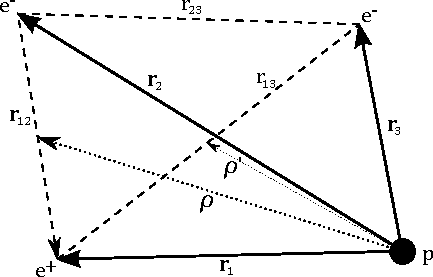
\includegraphics[height=2in]{PsHCoordinates}
	\caption{Positronium-hydrogen coordinate system}
	\label{fig:PsHCoords}
\end{figure}

We are investigating low-energy elastic ground-state Ps with ground-state hydrogen, Ps(1s)+H(1s), for energies up to the excitation threshold of Ps(n=2)+H(1s) at an energy of $\tfrac{3}{16}$ au ($5.102$ eV). Previous work on Ps-H scattering used the Kohn and inverse Kohn approach \cite{VanReeth2003, VanReeth2004}. The complex Kohn methods are more stable and suffer less from Schwartz singularities than the Kohn, inverse Kohn and generalized Kohn methods \cite{Lucchese1989,Cooper2009,Cooper2010}. Work by Van Reeth and Humberston on e$^+$-He scattering also used the complex Kohn variational method \cite{VanReeth1999}. The results presented in Sec. \ref{sec:Results} use the \emph{S} matrix complex Kohn method, but we present a general wavefunction that can be used in any of the variants of the Kohn variational method, as we describe in Sec. \ref{sec:Kohn}.

For S-wave Ps(1s)-H(1s) elastic scattering, the flexible complex-valued scattering wavefunction is given by
\begin{equation}
\Psi_0^{\pm,t} = \bar{S_0} + L_0^{\pm,t} \, \bar{C}_0 + \sum_{i=1}^{N(\omega)} c_i \phi_{i1},
\label{eq:TrialWave}
\end{equation}
where the superscript $t$ indicates that this is a trial wavefunction. The plus sign indicates the spatially symmetric singlet, and the minus sign indicates the spatially antisymmetric triplet case. The total orbital angular momentum of the system is equal to the orbital angular momentum of the incoming ground-state Ps, $\ell$. For partial waves $\ell > 0$,
\begin{equation}
\Psi_\ell^{\pm,t} = \bar{S}_\ell + L^{\pm,t}_\ell \, \bar{C}_\ell + \sum_{i=1}^{N(\omega)} c_{i,\ell} \phi_{i1} + \!\!\!\sum_{i=N(\omega)+1}^{2N(\omega)} \!\! d_{i,\ell} \phi_{i2}.
\label{eq:TrialWaveHigher}
\end{equation}
The scattering wavefunctions contain both the long-range terms $\bar{S}$ and $\bar{C}$ and the short-range correlation terms $\phi_{i1}$ for small interparticle distances. We show the coordinate system for Ps-H in Fig. \ref{fig:PsHCoords}. The vector $\rho$ is the position vector of the center of mass of the Ps atom with respect to the proton, i.e. $\vec{\rho} = \frac{1}{2}\left(\vec{r_1} + \vec{r_2}\right)$. The long-range terms of Eqs. (\ref{eq:TrialWave}) and (\ref{eq:TrialWaveHigher}) are given by
\begin{equation}
\label{eq:SCPhiDef}
\begin{bmatrix}
\widetilde{S}_\ell \\ \widetilde{C}_\ell
\end{bmatrix} = \textbf{u}  \begin{bmatrix}
\bar{S}_\ell \\ \bar{C}_\ell
\end{bmatrix} = \begin{bmatrix}
u_{00} & u_{01} \\  u_{10} & u_{11}
\end{bmatrix}
\begin{bmatrix}
\bar{S}_\ell \\ \bar{C}_\ell
\end{bmatrix}, 
\end{equation}
with
\begin{subequations}
\label{eq:SCBarPhiDef}
\begin{align}
\bar{S}_\ell &= \frac{1\pm P_{23}}{\sqrt{2}}Y_{\ell 0}(\theta_\rho,\varphi_\rho)\Phi_{Ps,1S}\left(r_{12}\right) \Phi_{H,1S}\left(r_3\right) \sqrt{2\kappa} \,j_\ell\left(\kappa\rho\right) \text{ and} \label{eq:SBar} \\
\bar{C}_\ell &= \frac{1\pm P_{23}}{\sqrt{2}}Y_{\ell 0}(\theta_\rho,\varphi_\rho)\Phi_{Ps,1S}\left(r_{12}\right) \Phi_{H,1S}\left(r_3\right) \sqrt{2\kappa} \,n_\ell\left(\kappa\rho\right) f_\ell(\rho). \label{eq:CBar}
\end{align}
\end{subequations}

$P_{23}$ is the exchange operator for the two electrons. $\Phi_{Ps,1s}\left(r_{12}\right)$ and $\Phi_{H,1s}\left(r_3\right)$ are the ground state wavefunctions of Ps and H, respectively. The shielding factor, $f_\ell(\rho)$, ensures that the singularity of the Neumann function is removed at the origin and is chosen to be
\begin{equation}
f_\ell(\rho) = \left[1 - \ee^{-\mu \rho} \left(1+\frac{\mu}{2}\rho\right)\right]^{m_\ell}.
\label{eq:PartialWaveShielding}
\end{equation}
The $m_\ell$ is an integer chosen for each $\ell$ so that $\bar{C}$ behaves like $\bar{S}$ as $\rho \rightarrow 0$.

We consider a number of variants of the Kohn variational method, described more fully in Sec. \ref{sec:Kohn}, and $\textbf{u}$ and $L^{\pm}_\ell$ take different forms depending on each. We use different $\textbf{u}$ matrices to generate multiple Kohn methods, namely the following:
\begin{subequations}
\label{eq:KohnU}
\begin{align}
&\text{generalized Kohn, } L^{\pm}_\ell = \tan(\delta^{\pm}_\ell-\tau), \textbf{u} = \left[ \begin{smallmatrix}
\cos \tau & \sin \tau \\  -\sin \tau & \cos \tau
\end{smallmatrix} \right], \label{eq:GenKohn}\\
&\text{generalized \emph{T} matrix Kohn, } L^{\pm,t}_\ell = T_\ell^{\pm\prime}, \textbf{u} = \left[ \begin{smallmatrix}
\cos\tau & \sin\tau \\ -\sin\tau + \ii \cos\tau & \cos\tau + \ii \sin\tau
\end{smallmatrix} \right], \text{and}\label{eq:GenTKohn} \\
&\text{generalized \emph{S} matrix Kohn, } L^{\pm,t}_\ell = S_\ell^{\pm\prime}, \textbf{u} = \left[ \begin{smallmatrix}
-\ii \cos\tau - \sin\tau & -\ii\sin\tau + \cos\tau \\ \ii\cos\tau - \sin\tau & \ii\sin\tau + \cos\tau
\end{smallmatrix} \right]. \label{eq:GenSKohn}
\end{align}
\end{subequations}
For the case of $\tau = 0$, these give the Kohn, the \emph{T} matrix and the \emph{S} matrix, respectively. $\tau = \frac{\pi}{2}$ in Eq. (\ref{eq:GenKohn}) gives the inverse Kohn. Note that our generalized \emph{T} matrix is different than Cooper et al.\ \cite{Cooper2010}, in that our $\bar{S}$ and $\bar{C}$ are swapped, which gives an outgoing wave. These are similar to the $\textbf{u}$ matrices given by Lucchese \cite{Lucchese1989} but are more generalized versions, and our \emph{T} matrix and \emph{S} matrix choices are a slightly different form.

The short-range terms are highly correlated Hylleraas-type functions, including all interparticle distances, given by
\begin{equation}
\label{eq:PhiDef}
\bar{\phi}_{ij} = \left(1 \pm P_{23}\right) Y_{\ell 0}(\theta_j,\phi_j) r_j^{\ell} r_1^{k_i} r_2^{l_i} r_{12}^{m_i} r_3^{n_i} r_{13}^{p_i} r_{23}^{q_i}
\end{equation}
The variable $\omega$ is a non-negative integer that determines the maximum number of terms in the basis set. For a chosen value of $\omega$, the integer powers of $r_i$ and $r_{ij}$ are constructed in such a way that 
\begin{equation}
k_i + l_i + m_i + n_i + p_i + q_i \leq \omega, \text{ with all } k_i, l_i, m_i, n_i, q_i \text{ and } p_i \geq 0.\end{equation}
The first symmetry in Eq. (\ref{eq:TrialWaveHigher}) has $j=1$ for $i=1$ to $N(\omega)$, and the second symmetry exists for $\ell > 0$, with $i = N(\omega)$ to $2N(\omega)$.

These short-range terms represent the angular momentum as being placed on either the positron ($r_1$) or on the electron on the Ps atom ($r_2$, and $r_3$ with exchange). Following up on the Ref. \cite{VanReeth2004} where the slow convergence of the $^3$P phase shift was discussed, we also tried a wavefunction where the angular momentum was placed on the electron of the H atom ($r_3$) and on the Ps ($\rho$). However, this did not improve convergence for us and was even marginally worse in some cases. The numerical techniques discussed in Sec. \ref{sec:Numerical} improved our convergence.

For partial waves with $\ell>1$, the orbital angular momentum could also be shared between both particles in the Ps atom \cite{Schwartz1961a}. An investigation of the contribution to the final results from each symmetry for e$^+$-He scattering \cite{VanReeth1997} has revealed that the mixed symmetries were not important, and because of the complexity of the analytical evaluation of the various matrix elements, we have omitted the mixed symmetry terms where angular momentum is shared.

% THE HAMILTONIAN
The Hamiltonian for the fundamental Coulombic system is
\begin{align}
H = -\frac{1}{2} \nabla_{r_1}^2 - \frac{1}{2} \nabla_{r_2}^2 - \frac{1}{2} \nabla_{r_3}^2 + \frac {1}{r_1}-\frac {1}{r_2}-\frac {1}{r_3}-\frac {1}{r_{12}}-\frac {1}{r_{13}}+\frac {1}{r_{23}},
\label{eq:Hamiltonian1}
\end{align}
which can also be expressed in Jacobi coordinates for Ps-H scattering as
\begin{align}
H = -\frac{1}{4} \nabla_{\rho}^2 - \frac{1}{2} \nabla_{r_3}^2 - \nabla_{r_{12}}^2 + \frac {1}{r_1}-\frac {1}{r_2}-\frac {1}{r_3}-\frac {1}{r_{12}}-\frac {1}{r_{13}}+\frac {1}{r_{23}}.
\label{eq:Hamiltonian2}
\end{align}


\subsection{Kohn Variational Methods}
\label{sec:Kohn}
This derivation follows a similar procedure as that of Refs.~\cite{Lucchese1989}, \cite{Cooper2010}, \cite{Armour1991}, and \cite{VanReethThesis}.
The functional for the full wavefunction in Eqs. (\ref{eq:TrialWave}) and (\ref{eq:TrialWaveHigher}) is (dropping the $\ell$ subscript and the $\pm$ superscript for clarity),
\begin{equation}
I[\Psi^t] = \left(\Psi^t, \mathcal{L} \Psi^t \right) = \int \Psi^t \mathcal{L} \Psi^t \,d\tau,
\label{eq:IlDefPsi}
\end{equation}
with
\beq
\mathcal{L} = 2(H - E).
\label{eq:LDef}
\eeq
Notice that the wavefunction is not conjugated, as pointed out by Cooper et al \cite{Cooper2010}. The total energy is given by
\begin{equation}
\label{eq:TotalEnergy}
E = \epsilon_H + \epsilon_{Ps} + \frac{1}{4}\kappa^2 = \epsilon_H + \epsilon_{Ps} + E_{\bm \kappa}.
\end{equation}

We assume the trial wavefunction is a small variation of the exact wavefunction $\Psi$, or
\beq
\Psi^t = \Psi + \delta \Psi
\label{eq:PsiTrialRelation}
\eeq
It can be shown that solving for $\delta I$, the variation of $I$, gives a result for the variational method of
\beq
\delta I = I[\Psi^t] - I[\Psi] = I[\Psi^t] = (L^t - L + I[\delta \Psi]) \det u.
\label{eq:IlPsiVariation}
\eeq
Here $L$ and $L^t$ correspond to the exact and trial wavefunctions, respectively. Neglecting the second order term in $\delta \Psi$ and realizing that $I[\Psi] = 0$, we get a functional for the variational $L^v$ of
\beq
L^v = L^t - I[\Psi^t] / \det u.
\label{eq:ComplexKohnVariation}
\eeq

Using the stationary property of the complex Kohn functional, we get
\beq
\frac{\partial L^v}{\partial L^t} = 0  \text{ and } \frac{\partial L^v}{\partial c_i} = 0 \text{ where $i = 1,\ldots,N$},
\label{eq:ComplexKohnStationary}
\eeq
which can be written as a matrix equation. For the S-wave, this is
\begin{equation}
\label{eq:ComplexKohnMatrix}
\begin{bmatrix} 
 (\widetilde{C},\mathcal{L}\widetilde{C}) & (\widetilde{C},\mathcal{L}\bar{\phi}_1) & \cdots & (\widetilde{C},\mathcal{L}\bar{\phi}_j) & \cdots\\
 (\bar{\phi}_1,\mathcal{L}\widetilde{C}) & (\bar{\phi}_1,\mathcal{L}\bar{\phi}_1) & \cdots & (\bar{\phi}_1,\mathcal{L}\bar{\phi}_j) & \cdots\\
 \vdots & \vdots & \ddots & \vdots \\
 (\bar{\phi}_i,\mathcal{L}\widetilde{C}) & (\bar{\phi}_i,\mathcal{L}\bar{\phi}_1) & \cdots & (\bar{\phi}_i,\mathcal{L}\bar{\phi}_j) & \cdots\\
 \vdots & \vdots & & \vdots & \\
\end{bmatrix}
\begin{bmatrix}
L^t\\
c_1\\
\vdots\\
c_i\\
\vdots
\end{bmatrix}
= -
\begin{bmatrix}
(\widetilde{C},\mathcal{L}\widetilde{S}) \\
(\bar{\phi}_1,\mathcal{L}\widetilde{S}) \\
\vdots \\
(\bar{\phi}_i,\mathcal{L}\widetilde{S}) \\
\vdots
\end{bmatrix}.
\end{equation}
This matrix equation can be rewritten as $\textbf{\emph{AX}}$ = -$\textbf{\emph{B}}$. For higher partial waves, the matrix equation looks the same but includes the second symmetry short-range terms. Finally, we solve for $L^v$, from which we obtain our phase shifts.
\begin{equation}
L^v = -\frac{1}{\det u} \left( \textbf{\emph{B}}^{tr} \textbf{\emph{X}} + (\widetilde{S},\mathcal{L} \widetilde{S}) \right)
\end{equation}
To determine the phase shifts, we use the relation given by Ref.~\cite{Lucchese1989} as
\begin{equation}
K_\ell = \tan \delta_\ell = (u_{01} + u_{11} L_\ell)(u_{00} + u_{10} L_\ell)^{-1}.
\end{equation}

%\begin{center}
%\line(1,0){250}
%\end{center}

\subsection{PsH Bound State and Optimization of Nonlinear Parameters}
As done earlier by Van Reeth and Humberston \cite{VanReeth2003,VanReeth2004}, we used the short-range correction part of the S-wave scattering wavefunction to compute the binding energy of $^1S$ PsH system. This allows us to determine the reliability of using our short-range terms for the Ps-H scattering problem. The wavefunction we use for the bound state is
\begin{equation}
\label{eq:BoundWavefn}
\Psi^\pm = \sum_{i=1}^{N(\omega)} c_i \phi_{1i}^\pm,
\end{equation}
where $\phi_{1i}^\pm$ is the same as in Eq. (\ref{eq:PhiDef}). The Rayleigh-Ritz method is used, and the optimization of the nonlinear parameters has been done using the both the Newton and simplex methods \cite{Yan1999,GSL}. For the $^3$S case and $\ell \neq 0$, even though there is not a bound state, we use the same method to optimize the nonlinear parameters to get the lowest energy. For $\ell > 0$, as in the scattering problem, the wavefunction includes both sets of short-range terms for this optimization. While not necessarily the optimum choice, these optimized nonlinear parameters are used in the scattering problem. There is an additional nonlinear parameter $\mu$ in the scattering problem that would be impractical to simultaneously optimize with these nonlinear parameters due to computational costs.

\subsection{Born Approximation}
The Born approximation to the \emph{K} matrix \cite{Bransden2003} is given by the first term in Eqs. (\ref{eq:TrialWave}) and (\ref{eq:TrialWaveHigher}). For the Kohn variational method, this leads to the Born approximation given by
\begin{equation}
\label{eq:Born}
\tan\delta_\ell \approx -(\widetilde{S}_\ell,\mathcal{L}\widetilde{S}_\ell )\, .
\end{equation}
We also consider a modified Born approximation that uses the long-range terms only in equations \ref{eq:TrialWave} and \ref{eq:TrialWaveHigher}.

\subsection{Cross Sections}
We calculate the integrated and differential elastic cross sections using \cite{Bransden2003}, respectively,
\begin{equation}
\label{eq:TotalCross}
\sigma_{el}^\pm = \frac{4}{\kappa^2} \sum_{\ell=0}^\infty (2\ell+1) \sin^2 \delta_\ell^\pm
\end{equation}
and
\begin{align}
\label{eq:DiffCross}
\nonumber \frac{d\sigma_{el}^\pm}{d\Omega} = \frac{1}{\kappa^2} & \sum_{\ell=0}^\infty \sum_{\ell^\prime=0}^\infty (2\ell+1)(2\ell^\prime+1) \exp\left\{\ii \left[\delta_\ell(\kappa) - \delta_{\ell^\prime}(\kappa) \right] \right\} \\
& \times \sin\delta_\ell^\pm(\kappa) \sin\delta_{\ell^\prime}^\pm(\kappa) P_\ell(\cos\theta) P_{\ell^\prime}(\cos\theta)\,.
\end{align}
Equation (\ref{eq:TotalCross}) is in units of $\pi a_0^2$, and Eq. (\ref{eq:DiffCross}) is in units of $\pi a_0^2 / \rm{sr}$. The singlet for each of the partial waves contributes $1/4$ to the integrated and differential cross sections, while the triplet contributes $3/4$.

The momentum transfer cross sections can be useful in plasma applications \cite{Wang2014, McEachran2014}. These cross sections have been measured for Ps with multiple atomic and molecular molecular targets \cite{Nagashima1998,Saito2003}. The momentum transfer cross sections are given by \cite{Bransden2003}
\begin{equation}
\label{eq:MomentumCross}
\sigma_{m}^\pm = \frac{4}{\kappa^2} \sum_{\ell=0}^\infty (\ell+1) \sin^2 (\delta_\ell^\pm - \delta_{\ell+1}^\pm) .
\end{equation}
The ortho-para conversion cross sections give the conversion of the projectile ortho-Ps to para-Ps by \cite{Hara1975}
\begin{equation}
\label{eq:OrthoParaCross}
\sigma_{c} = \frac{1}{4 \kappa^2} \sum_{\ell=0}^\infty (2 \ell+1) \sin^2 (\delta_\ell^+ - \delta_\ell^-).
\end{equation}


\subsection{Effective Range}

The scattering length is defined as \cite{Bransden2003}
\begin{equation}
\label{eq:ScatLen}
a_\ell^\pm = -\lim_{\kappa \to 0} \frac{\tan{\delta_\ell^\pm}}{\kappa^{2\ell+1}}.
\end{equation}
The Kohn variational methods give an exact upper bound on the scattering length \cite{Joachain1979}. The scattering length can give information about whether there is a bound state in the system, and at zero energy \cite{Buckman1989},
\begin{equation}
\label{eq:ScatLenCross}
\sigma_m = \sigma_{el} = 4 a^2 .
\end{equation}

For short-range potentials, the effective range $r_0$ is given by \cite{Bethe1949,Blatt1949}
\begin{equation}
\label{eq:EffectiveRangeShort}
\kappa \cot\delta_0^\pm = -\frac{1}{a_0^\pm} + \frac{1}{2} r_0^\pm \kappa^2.
\end{equation}
The effective range is a measure of the interaction region of the scattering problem. This is the fitting used throughout the literature \cite{Ivanov2002,VanReeth2003,Blackwood2002,Walters2004}. As pointed out in Ref. \cite{Fabrikant2014}, the van der Waals interaction should be taken into account for low-energy Ps-atom scattering. An ERT expansion for the van der Waals interaction is given by \cite{Drake2006}
\begin{equation}
\label{eq:EffectiveRangeLongAu}
\kappa \cot\delta_0^\pm = -\frac{1}{a} + \frac{1}{2} r_0^\pm \kappa^2 - \frac{4 \pi C}{15 a^2} \kappa^3 - \frac{16 C}{15 a} \kappa^4 \ln \left(\kappa \right).
\end{equation}
We use the van der Waals coefficient, C, given by Martin and Fraser as 34.78473 au \cite{Martin1980}.

Gao has developed a quantum defect theory (QDT) treatment, solving the Schr\"{o}dinger equation for an attractive $r^{-6}$ potential to find an expression relating the phase shifts to a quantity he refers to as $K_l^0(E_{\bm \kappa})$ \cite{Gao1998}.
\begin{equation}
\label{eq:GaoZEqn}
\tan\delta_l = [Z_{ff} - K_l^0(E_{\bm \kappa}) Z_{gf}]^{-1} [K_l^0(E_{\bm \kappa}) Z_{gg} - Z_{fg}]
\end{equation}
The Z functions in this equation are described fully in his paper. The phase shifts are fitted to Eq. (\ref{eq:GaoZEqn}) to determine $K_l^0(E)$ for each $\kappa$ value. $K_l^0(\epsilon)$ must be expanded in a Taylor series as
\begin{equation}
\label{eq:GaoKTaylor}
K_l^0(E_{\bm \kappa}) = K_l^0(0) + {K_l^0}^\prime(0) E_{\bm \kappa} + \ldots.
\end{equation}
From this, $K_l^0(0)$ and ${K_l^0}^\prime(0)$ are determined. $K_l^0(0)$ slowly varies with the energy $E_{\bm \kappa}$, and ${K_l^0}^\prime(0)$ gives the quickly varying part. In Ref. \cite{Gao1998a}, Gao performed an expansion of this expression for low $\kappa$ to generate expressions for $a_\ell$ and $r_0$:

\begin{equation}
\label{eq:GaoScatLenS}
a_{\ell=0} = \frac{2\pi}{[\Gamma(1/4)]^2} \frac{K_{l=0}^0(0) - 1}{K_{l=0}^0(0)} \beta_6
\end{equation}

\begin{equation}
\label{eq:GaoScatLenP}
a_{\ell=1} = -\frac{\pi}{18[\Gamma(1/4)]^2} \frac{K_{l=1}^0(0) + 1}{K_{l=1}^0(0)} \beta_6^3
\end{equation}

\begin{equation}
\label{eq:GaoEffRange}
r_{\ell=0} = \frac{[\Gamma(1/4)]^2}{3\pi} \frac{[K_{l=0}^0(0)]^2 + 1}{[K_{l=0}^0(0) - 1]^2} \beta_6 + \frac{[\Gamma(1/4)]^2}{\pi} \frac{{K_{l=0}^0}^\prime(0)^2(\hbar^2/2\mu)(1/\beta_6)^2}{[K_{l=0}^0(0) - 1]^2} \beta_6.
\end{equation}
The term $\beta_6$ is related to $C$ by $\beta_6 = (2\mu C/\hbar^2)^{1/4}$.

Lastly, we use an expression from Ref. \cite{Blackwood2002} to get an estimate of the $^1$S effective range, given by
\begin{equation}
\label{eq:BlackwoodERT}
r_0^+ = \frac{a_0^+ \sqrt{4 E_b} - 1}{2 a_0^+ E_b}.
\end{equation}
No equivalent expression exists for $r_0^-$, as there is not a $^3$S bound state.


\section{Numerics}
\label{sec:Numerical}
%Describe Todd's procedure.
%How terms are eliminated for the bound-state
%and give the procedure for determining the
%number for the scattering.
%Give a table for the number of terms for bound-state,
%for singlet and triplet scattering.
%Compare with the total number of terms,
%and the number of terms that Peter considered.
%Explain how the non-linear terms are obtained for the
%bound-state, singlet and triplet scattering.
%\todoi{Compare with the nonlinear parameters that Peter used.}
%\vskip 1truecm
%\noindent

\subsection{Short-Short Integrations}
\label{sec:ShortInt}
For the PsH bound state and $^{1,3}S$ Ps(1s)-H(1s) elastic scattering, we use the efficient asymptotic expansion method presented by Drake and Yan \cite{Drake1995} for the evaluation of correlated integrals of the form
\begin{equation}
\label{eq:ShortInt}
I(j_1,j_2,j_3,j_{12},j_{23},j_{31}; \bar{\alpha}, \bar{\beta}, \bar{\gamma}) =
\int
d \textbf{r}_1 d \textbf{r}_2 d \textbf{r}_3
r_1^{j_1} r_2^{j_2} r_3^{j_3} r_{12}^{j_{12}}
r_{23}^{j_{23}} r_{31}^{j_{31}}
e^{-(\bar{\alpha} r_1 + \bar{\beta} r_2 + \bar{\gamma} r_3)}\, .
\end{equation}
These integrals arise from evaluation of the matrix elements $(\phi_i, L \phi_j)$, $(\phi_i, H \phi_j)$ and $(\phi_i, \phi_j)$, where $H$ is the full Hamiltonian given in Eqs. \ref{eq:Hamiltonian1} and \ref{eq:Hamiltonian2}. To verify our calculation of these integrals for the S-wave and P-wave, we also use the recursion relations of Pachucki \cite{Pachucki2004}.

For $\ell > 0$, we use two different methods to perform these integrations. The first is the method used by Van Reeth \cite{VanReethThesis}. In this method, we rotate and then integrate over external angles, reducing these integrals down to the form of Eq. (\ref{eq:ShortInt}). We then use the asymptotic expansion method \cite{Drake1995} to solve. This works through the D-wave, as the integrals become too singular for $\ell > 2$. For all partial waves, we can use a more general method from Yan and Drake \cite{Yan1997}. This C code for the second method is slower but has been used mainly for $l > 2$, through the H-wave. These integrals have the form of
\begin{align}
\label{eq:ShortIntGen}
\nonumber I(\ell_1^\prime m_1^\prime, & \ell_2^\prime m_2^\prime, \ell_3^\prime m_3^\prime; j_1,j_2,j_3,j_{12},j_{23},j_{31}; \bar{\alpha}, \bar{\beta}, \bar{\gamma}) \\
\nonumber = & \int
d \textit{\textbf{r}}_1 d \textit{\textbf{r}}_2 d \textit{\textbf{r}}_3
r_1^{j_1} r_2^{j_2} r_3^{j_3} r_{12}^{j_{12}}
r_{23}^{j_{23}} r_{31}^{j_{31}}
e^{-(\bar{\alpha} r_1 + \bar{\beta} r_2 + \bar{\gamma} r_3)} \\
& \times Y_{\ell_1^\prime m_1^\prime}^* (\textit{\textbf{r}}_1) Y_{\ell_2^\prime m_2^\prime}^* (\textit{\textbf{r}}_2) Y_{\ell_3^\prime m_3^\prime}^* (\textit{\textbf{r}}_3)
Y_{\ell_1 m_1} (\textit{\textbf{r}}_1) Y_{\ell_2 m_2} (\textit{\textbf{r}}_2) Y_{\ell_3 m_3} (\textit{\textbf{r}}_3)\, .
\end{align}

\subsection{Long-Range Integrations}
\label{sec:LongInt}
We evaluate the long-range--long-range and short-range--long-range matrix elements in Eq. (\ref{eq:ComplexKohnMatrix}) using the standard Gauss-Laguerre and Gauss-Legendre quadratures. Due to the cusp at $r_1 = r_2$ and $r_2 = r_3$ in the integrands, we split the $r_2$ and $r_3$ integrations into Gauss-Legendre quadratures before the cusp and Gauss-Laguerre after the cusp. Previous calculations \cite{VanReeth2003,VanReeth2004} treated these cusps as unimportant by 25 au, while we have extended it to 100 au before we consider them unimportant. We find that this increases the convergence of the matrix elements.

To further improve the convergence of the short-range--long-range matrix elements, we investigate the integrands. The biggest source of difficulty in converging these results comes through the Gaussian-Laguerre quadratures in the $r_1$, $r_2$ and $r_3$ integrations -- especially $r_1$. We increase the number of integration points to more than seven times as many in previous work \cite{VanReeth2003,VanReeth2004} to better represent the integrands. This brute force approach can increase the computational time greatly, so we take another approach to further increase the accuracy. Specifically, the tails of the integrands are negligible, and the integrand closer to the origin is not represented adequately. To resolve this, for each of the Gauss-Laguerre quadratures, we introduce an extra $e^{-\lambda r_i}$ and remove it with $e^{\lambda r_i}$ after the quadrature, bringing the abscissae closer to the origin without increasing the number of integration points. For further details on integrations, refer to Ref. \cite{Woods2015}.
%\todoi{Put in convergence information from ``D:/Denton/Dropbox/Research/Peter Files/D-Wave Notes/NotesonIntegrationJan2013.pdf''}

\subsection{Todd's procedure}
\label{sec:Todd}
We use a method from Todd \cite{Todd2007} to remove short-range terms that contribute to linear dependence. This is a variation of the procedure from L\"uchow and Kleindienst \cite{Luchow1992}. They use multiple blocks, while we optimize with a single block. They also use a criteria of $\Delta E$ to determine when to discard terms. Instead, we compare the lowest eigenvalues from the separate calculations using the upper and lower triangular matrices in LAPACK's \texttt{dsygv} routine \cite{LAPACK}, discarding terms when they cause the difference to be greater than a predetermined threshold. We refer here to the reordering introduced by this method as ``Todd ordering'', as compared to the original ordering indicated by increasing $\omega$. The summation limits in Eqs. (\ref{eq:TrialWave}) and (\ref{eq:TrialWaveHigher}) are then indicated by $N^\prime(\omega)$ instead of $N(\omega)$ to indicate that this is not the full set described after Eq. (\ref{eq:PhiDef}). When we do convergence checks via extrapolations, we put the terms back in the original ordering but with the set of $N^\prime(\omega)$ terms.

\subsection{Selection of Short-Range Terms}
\label{sec:Truncation}
We observe that the short-range terms used in the same order as the output of the Todd algorithm will generate better-converged phase shifts, and we can include more short-range terms before linear dependence becomes a problem. The phase shifts are calculated using this set of short-range terms for the generalized Kohn variational method for multiple $\tau$ values in Eq. (\ref{eq:KohnU}). We further truncate this basis set where the phase shifts for the different Kohn methods begin to diverge, as seen in Fig. \ref{fig:swave-phase-divergence}. The results in Sec. \ref{sec:Results} use the \emph{S} matrix complex Kohn with this set of short-range terms.

\begin{figure}[H]
	\centering
	\includegraphics[width=3.3in]{swave-phase-divergence}
	\caption{(Color online) Divergence of the $^1$S phase shifts with respect to number of short-range terms}
	\label{fig:swave-phase-divergence}
\end{figure}

For $^1$S, we noticed an additional property of the phase shift graphs. When $\delta_0^+$ is plotted for one Kohn method with respect to $N(\omega)$ for multiple $\mu$ values ($\mu$ defined in Eq. (\ref{eq:PartialWaveShielding})), the phase shifts agree well for the different $\mu$ values up until linear dependence becomes apparent visually. We used this criteria to determine where to truncate the basis set, stopping at 1505 terms for $^1S$. We did not see a similar effect for $^3$S or other partial waves.

\subsection{Fittings}
As with the previous Kohn calculation of Van Reeth and Humberston \cite{VanReeth2004}, we fit our computed phase shifts for the S-wave and P-wave to the resonance formula
\begin{equation}
\label{eq:ResonanceFit}
\delta(E_{\bm \kappa}) = A + B E_{\bm \kappa} + C E_{\bm \kappa}^2 + \arctan \left[ \frac{^1\Gamma}{2(^1E_R - E_{\bm \kappa})} \right] + \arctan \left[ \frac{^2\Gamma}{2(^2E_R - E_{\bm \kappa})} \right]
\end{equation}
to extract out the positions ($^1E_R$ and $^2E_R$) and widths
($^1\Gamma$ and $^2\Gamma$) of the two resonances. 
This formula is comprised of the Breit-Wigner resonance
terms \cite{Bransden2003} for the two resonances and allows for a slowly varying polynomial
background. The $^1$D and $^1$F resonance fits are performed without the second $\arctan$ term, as they have a single resonance. 
The data from each variant of the Kohn variational methods was fitted using the MATLAB \cite{MATLAB} nonlinear fitting routine \texttt{nlinfit} with eight possible weightings.
For each variant of the Kohn variational method, the four parameters were determined for each of the eight fits and compared.

For each variant of the Kohn variational method, we extrapolated the phase shifts in Tables \ref{tab:SWaveSingletPhase}, \ref{tab:SWaveTripletPhase}, and \ref{tab:SWaveSingletPhase} according to the empirical formula \cite{VanReeth2003}
\begin{equation}
\label{eq:Extrap}
\tan\delta_\ell^\pm(\omega) = \tan\delta_\ell^\pm(\omega\to\infty) + \frac{c}{\omega^p}\, .
\end{equation}
We use these extrapolated values to estimate the convergence of our phase shifts and the error in our final results.
A similar method is used to extrapolate the scattering lengths by fitting to
\begin{equation}
\label{eq:ExtrapA}
a_\ell^\pm(\omega) = a_\ell^\pm(\omega\to\infty) + \frac{d}{\omega^q}\, .
\end{equation}
The difference between the scattering length and the extrapolated scattering length is considered the error in tables \ref{tab:SWaveScatLenERT} and \ref{tab:PWaveScatLen}. No convergence pattern was found for the effective range.

\subsection{Nonlinear Parameters and Terms Used}
\label{sec:Parameters}

\begin{table}[H]
  \centering
	\begin{ruledtabular}
    \begin{tabular}{cccccccccc}
    Param. & $^1$S & $^3$S & $^1$P & $^3$P & $^1$D & $^3$D & $^{1,3}$F & $^{1,3}$G & $^{1,3}$H \\
    \colrule
	$\omega$           & 7     & 7     & 7     & 7     & 6     & 6     & 5    & 5   & 5 \\
	$N^\prime(\omega)$ & 1505  & 1633  & 1000  & 1000  & 916   & 919   & 462  & 462 & 462 \\
	$\alpha$           & 0.586 & 0.323 & 0.397 & 0.310 & 0.359 & 0.356 & 0.5  & 0.5 & 0.5 \\
	$\beta$            & 0.580 & 0.334 & 0.376 & 0.311 & 0.368 & 0.365 & 0.6  & 0.6 & 0.6 \\
	$\gamma$           & 1.093 & 0.975 & 0.962 & 0.995 & 0.976 & 0.976 & 1.1  & 1.1 & 1.1 \\
	$\mu$              & 0.9   & 0.9   & 0.9   & 0.9   & 0.7   & 0.7   & 0.7  & 0.7 & 0.7 \\
	$m_\ell$           & 1     & 1     & 3     & 3     & 7     & 7     & 7    & 9   & 11 \\
    \end{tabular}
  \end{ruledtabular}
  \caption{Parameters for each partial wave}
  \label{tab:Nonlinear}
\end{table}

\section{Results}
\label{sec:Results}

\subsection{Bound State Results}

The PsH bound state calculation was performed to determine the reliability of the short-range part of the wavefunction to describe Ps-H scattering at small distances. The Rayleigh-Ritz variational method provides a true bound on the total and binding energies, which converge well with respect to $\omega$. To be consistent with the scattering calculation, we report the results obtained with the same set of nonlinear parameters that we use in the scattering calculation, as given in Table \ref{tab:Nonlinear}. We note that we are able to obtain a slightly better value for the binding energy with higher $\omega$, but we are unable to use this many terms in the full scattering calculations for Ps-H. Table \ref{tab:BoundEnergy} compares our energies for PsH with that obtained by other groups.

Our calculation yields a better value for these
quantities than the earlier variational calculation \cite{VanReeth2003,VanReeth2004}
but not as good as the variational calculation of
Yan and Ho \cite{Yan1999}, who also used Hylleraas wave functions.
While we do not obtain the best value of the binding energy
(this was not the purpose of our calculation),
we obtained results for this quantity which compare favorably with
the most elaborate calculation in the literature, which
used 5000 ECGs \cite{Bubin2006}.
Our calculation of the binding energy gives us some confidence
in the reliability of the short-range part of the
scattering wave function to describe
the $^1S$ PsH system.

\squeezetable  % Makes the table smaller
\begin{table}[H]
\begin{center}1
%\begin{tabular}{|l|l|c|l|l|}
\begin{ruledtabular}  % From http://www.latex-community.org/forum/viewtopic.php?f=45&t=20722
\begin{tabular}{l l c l l}
%\toprule
Group & Method & Terms & Total Energy (au) & Binding Energy (eV)\\
%\hline
\colrule
%\midrule
Current work & Variational with Hylleraas & 1505 & -0.789 189 725 & 1.066 406 705 \\
Van Reeth (2003) \cite{VanReeth2003} & Variational with Hylleraas $(\omega = 6)$ & 721 & -0.789 156 & 1.065 5$^\star$ \\
Ho (1986) \cite{Ho1986} & Variational with Hylleraas & 396 & -0.788 945$^\star$ & 1.059 75 \\
Yan (1999) \cite{Yan1999} & Variational with Hylleraas $(\omega \rightarrow \infty)$ & --- & -0.789 196 714 7$^\star$ & 1.066 596 896 \\
Blackwood (2002) \cite{Blackwood2002} & CC 14Ps14H & --- & -0.786 5 & 0.994$^\star$ \\
Walters (2004) \cite{Walters2004} & CC 14Ps14H + $\text{H}^-$ & --- & -0.787 9 & 1.03$^\star$\\
Mitroy (2006) \cite{Mitroy2006} & ECGs with SVM & 1800 & -0.789 196 740$^\star$ & 1.066 597 58 \\
Bubin (2006) \cite{Bubin2006} & ECGs variational & 5000 & -0.789 196 765 251$^\star$ & 1.066 598 271 959 \\
%\bottomrule
\end{tabular}
\end{ruledtabular}
\caption{Positronium hydride energy comparisons. The values marked by an asterisk are the reported values, and the other values are obtained by using the conversion factor given in Ref. \cite{Mohr2012,*NISTConversions}.}
\label{tab:BoundEnergy}
\end{center}
\end{table}

\subsection{Phase Shifts and Cross Sections}

In Tables \ref{tab:SWaveSingletPhase} and \ref{tab:SWaveTripletPhase}, we show the $^{1,3}$S phase shifts using the \emph{S} matrix complex Kohn variational method. To the accuracy given, the results agree from the various methods described in Sec. \ref{sec:Kohn}, after removing any obvious Schwartz singularities. We compute extrapolated values from $\omega = 4$ to $\omega = 7$ to estimate the phase shifts as $\omega \rightarrow \infty$ using Eq. (\ref{eq:Extrap}). By computing the percentage difference between the extrapolated phase shifts and the computed phase shifts at $\omega=7$, we estimate that the $^1$S phase shifts have converged to better than about $0.22\%$ for the range $\kappa=0.1$ to $0.7$ and that the $^3$S phase shifts have converged to better than $0.27\%$ for the same range of $\kappa$.

In this table, we also compare our results with the earlier Kohn variational results \cite{VanReeth2003,VanReeth2004} and with the elaborate CC results of Walters' group \cite{Blackwood2002,Walters2004}. The current $\omega = 7$ results are in excellent agreement with the earlier Kohn $\omega = 6$ variational results, being either identical or slightly lower, indicating that the earlier S-wave calculations were well-converged. The slight difference in phase shifts between the previous and current Kohn methods can be attributed to two factors. Using Todd's procedure (described in Sec. \ref{sec:Todd}) allows us to use more terms (see Table \ref{tab:Nonlinear}) than the earlier Kohn calculations \cite{VanReeth2003,VanReeth2004}, which used 721 terms. This slightly increased the phase shifts, but we also use more integration points in these calculations, which have the effect of slightly decreasing the phase shifts.

The complex Kohn results are in good agreement with the CC results of the Walters group \cite{Blackwood2002,Walters2004}. For the singlet, the complex Kohn phase shifts are slightly larger than the CC results. Because of the empirical bounds on the Kohn variational results and, in practice on the CC (except for the Buttle correction), the complex Kohn results could be slightly more accurate than the CC.
The situation is reversed for the triplet. In this case, the Kohn results are slightly more negative than the CC results; however, the complex Kohn and CC results are in very good agreement.

The recent CVM S-wave results from Zhang and Yan \cite{Zhang2012} agree extremely well with the Kohn results, even for the triplet. Figure \ref{fig:spd-wave-phases}(a) compares our complex Kohn phase shifts over the energy range up to the Ps(n=2) threshold with the CC and CVM results. Excellent agreement between the three sets of results is evident. In Fig. \ref{fig:swave-comparisons}, we compare the $^{1,3}$S phase shifts obtained from the complex Kohn variational method with various other calculations.

Tables \ref{tab:PWavePhase} and \ref{tab:DWavePhase} give the $^{1,3}$P and $^{1,3}$D phase shifts that we determine using the complex Kohn variational method. The small percentage differences with the extrapolated values for the P-wave indicates that our phase shifts are well converged. Similar to the $^{1,3}$S, the $^1$P phase shifts are slightly above the CC results, and our $^3$P phase shifts are below. Figure \ref{fig:spd-wave-phases}(b) shows that the complex Kohn and CC results agree well.

We have had difficulty performing extrapolations on the D-wave phase shifts. For $\kappa = 0.2 - 0.7$, the percentage difference between the $^1$D extrapolations and $\omega = 6$ results is less than $11\%$. The percentage differences for $^3$D for the same range are less than $23\%$, with the exception of $\kappa = 0.4$. This has a larger percentage difference of $48.7\%$, and this is also where the $^3$D phase shifts go from positive to negative. It should be noted that the extrapolation is an empirical fit. The $\omega = 5$ and $\omega = 6$ phase shifts differ by no more than 8.6\% for $^1$D and 10.3\% for $^3$D. Both the $^1$D and $^3$D phase shifts are below the CC, though Fig. \ref{fig:spd-wave-phases}(c) shows that the complex Kohn and CC also agree reasonably well. The phase shifts are small for $^3$D, and its contribution to the total cross sections given in Fig. \ref{fig:combined-cross-sections} is small.


\begin{table}[H]
\centering
\begin{ruledtabular}
\begin{tabular}{c c c c c c c}
$\kappa$ (au) & $\delta_0^+ (\omega = 7)$ & $\delta_0^+ (\omega \rightarrow \infty)$ & \% Diff$^+$ & $\delta_0^+$ (Kohn) \cite{VanReeth2003} & $\delta_0^+$ (CC 14Ps14H+H$^-$) \cite{Walters2004} & $\delta_0^+$ (CVM) \cite{Zhang2012} \\
\colrule
0.1 & -0.427 & -0.426 & 0.223\% & -0.427 & -0.432 & -0.42636 \\
0.2 & -0.820 & -0.819 & 0.010\% & -0.820 & -0.833 & -0.81973 \\
0.3 & -1.161 & -1.161 & 0.040\% & -1.161 & -1.179 & --- \\
0.4 & -1.446 & -1.446 & 0.022\% & -1.446 & -1.466 & --- \\
0.5 & -1.678 & -1.677 & 0.031\% & -1.677 & -1.699 & --- \\
0.6 & -1.858 & -1.857 & 0.040\% & -1.857 & -1.884 & --- \\
0.7 & -1.964 & -1.963 & 0.045\% & -1.964 & -2.012 & --- \\
\end{tabular}
\end{ruledtabular}
\caption{$^1$S phase shifts. \% Diff$^+$ is the percent difference between the current Kohn $\omega = 7$ and $\omega \rightarrow \infty$ results. CC is the close coupling method, and CVM is the confined variational method.}
\label{tab:SWaveSingletPhase}
\end{table}

\begin{table}[H]
\centering
\begin{ruledtabular}
\begin{tabular}{c c c c c c c}
$\kappa$ (au) & $\delta_0^- (\omega = 7)$ & $\delta_0^- (\omega \rightarrow \infty)$ & \% Diff$^-$ & $\delta_0^-$ (Kohn) \cite{VanReeth2003} & $\delta_0^-$ (CC 14Ps14H) \cite{Blackwood2002} & $\delta_0^-$ (CVM) \cite{Zhang2012} \\
\colrule
0.1 & -0.215 & -0.214 & 0.120\% & -0.214 & -0.206 & -0.21464 \\
0.2 & -0.431 & -0.431 & 0.063\% & -0.432 & -0.414 & -0.43159 \\
0.3 & -0.645 & -0.645 & 0.094\% & -0.645 & -0.624 & --- \\
0.4 & -0.850 & -0.849 & 0.130\% & -0.850 & -0.838 & --- \\
0.5 & -1.041 & -1.040 & 0.166\% & -1.040 & -1.037 & --- \\
0.6 & -1.217 & -1.214 & 0.273\% & -1.215 & -1.213 & --- \\
0.7 & -1.375 & -1.372 & 0.250\% & -1.373 & -1.367 & --- \\
\end{tabular}
\end{ruledtabular}
\caption{$^3$S phase shifts. \% Diff$^-$ is the percent difference between the current Kohn $\omega = 7$ and $\omega \rightarrow \infty$ results.}
\label{tab:SWaveTripletPhase}
\end{table}

\begin{table}[H]
\begin{center}
\begin{ruledtabular}
\begin{tabular}{c c c c c c c c c c}
$\kappa$ (au) & $\delta_1^+ (\omega = 7)$ & $\delta_1^+ (\omega \rightarrow \infty)$ & \% Diff$^+$ & $\delta_1^+$ (CC) \cite{Walters2004} & $\delta_1^- (\omega = 7)$ & $\delta_1^- (\omega \rightarrow \infty)$ & \% Diff$^-$ & $\delta_1^-$ (CC) \cite{Blackwood2002} \\
\colrule
0.1 & $0.226^{-1}$ & $0.227^{-1}$ & $0.465\%$ & $0.221^{-1}$ & $-0.178^{-2}$ & $-0.172^{-2}$ & $3.176\%$ & $-0.953^{-3}$ \\
0.2 & $0.191$      & $0.192$      & $0.306\%$ & $0.183$      & $-0.167^{-1}$ & $-0.165^{-1}$ & $0.993\%$ & $-0.122^{-1}$ \\
0.3 & $0.609$      & $0.611$      & $0.314\%$ & $0.580$      & $-0.552^{-1}$ & $-0.540^{-1}$ & $0.749\%$ & $-0.456^{-1}$ \\
0.4 & $0.994$      & $0.996$      & $0.205\%$ & $0.956$      & $-0.115$      & $-0.114$      & $0.698\%$ & $-0.104$ \\
0.5 & $1.140$      & $1.142$      & $0.140\%$ & $1.106$      & $-0.183$      & $-0.182$      & $0.749\%$ & $-0.178$ \\
0.6 & $1.162$      & $1.163$      & $0.137\%$ & $1.134$      & $-0.248$      & $-0.246$      & $0.896\%$ & $-0.247$ \\
0.7 & $1.152$      & $1.154$      & $0.181\%$ & $1.133$      & $-0.292$      & $-0.281$      & $1.237\%$ & $-0.295$ \\
\end{tabular}
\end{ruledtabular}
\caption{$^{1,3}$P phase shifts}
\label{tab:PWavePhase}
\end{center}
\end{table}


\begin{table}[H]
\begin{center}
\begin{ruledtabular}
\begin{tabular}{c c c c c}
$\kappa$ (au) & $\delta_2^+ (\omega = 6)$ & $\delta_2^+$ (CC 14Ps14H+H$^-$) \cite{Walters2004} & $\delta_2^- (\omega = 6)$ & $\delta_2^-$ (CC 14Ps14H) \cite{Blackwood2002} \\
\colrule
$0.1$ & $1.358^{-4}$ & $1.46^{-4}$ & $5.808^{-5}$ & $8.48^{-5}$ \\
$0.2$ & $2.987^{-3}$ & $3.15^{-3}$ & $7.120^{-4}$ & $1.15^{-3}$ \\
$0.3$ & $1.592^{-2}$ & $1.65^{-2}$ & $1.065^{-3}$ & $2.84^{-3}$ \\
$0.4$ & $4.933^{-2}$ & $4.95^{-2}$ & $-2.002^{-3}$ & $2.37^{-3}$ \\
$0.5$ & $1.113^{-1}$ & $1.08^{-1}$ & $-1.122^{-2}$ & $-4.66^{-3}$ \\
$0.6$ & $2.027^{-1}$ & $1.94^{-1}$ & $-2.647^{-2}$ & $-1.85^{-2}$ \\
$0.7$ & $3.215^{-1}$ & $3.02^{-1}$ & $-4.451^{-2}$ & $-3.27^{-2}$ \\
\end{tabular}
\end{ruledtabular}
\caption{$^{1,3}$D phase shifts}
\label{tab:DWavePhase}
\end{center}
\end{table}



% Caption idea from http://tex.stackexchange.com/questions/102925/how-can-i-insert-the-symbols-into-the-caption-of-a-figure
% Could also do similar caption to Laricchia's paper (doi:10.1088/1742-6596/194/1/012036)
\begin{figure}[H]
	\centering
	\includegraphics[width=3.3in]{swave-comparisons}
	\caption{(Color online) Comparison of $^1$S (a) and $^3$S (b) phase shifts with results from other groups. Results are ordered according to year of publication. This work -- solid curves; \mbox{\textcolor{blue}{$\times$} -- CC \cite{Walters2004};} \mbox{$\CIRCLE$ -- Kohn \cite{VanReeth2003};} \mbox{\textcolor{red}{\textbf{+}} -- CC \cite{Blackwood2002};} \mbox{$\blacktriangle$ -- Chiesa 2002 \cite{Chiesa2002};} \mbox{$\triangledown$ -- SVM 2002 \cite{Ivanov2002};} \mbox{$\Circle$ -- SVM 2001 \cite{Ivanov2001};} \mbox{\textcolor{red}{$\vartriangle$} -- Sinha 2000 \cite{Sinha2000};} \mbox{$\blacksquare$ -- Adhikari 1999 \cite{Adhikari1999};} \mbox{$\square$ -- Campbell 1998 \cite{Campbell1998};} \mbox{$\vartriangle$ -- Sinha 1997 \cite{Sinha1997};} \mbox{\textcolor[RGB]{0,127,0}{$\bigstar$} -- Ray 1997 \cite{Ray1997};} \mbox{$\triangleright$ -- Drachman 1976 \cite{Drachman1976};} \mbox{\textcolor{red}{$\blacklozenge$} -- Drachman 1975 \cite{Drachman1975};} \mbox{\textcolor{blue}{$\lozenge$} -- Hara 1975 \cite{Hara1975};} \mbox{$\blacktriangledown$ -- Fraser 1961 \cite{Fraser1961}.}}
	\label{fig:swave-comparisons}
\end{figure}


\begin{figure}[H]
	\centering
	\includegraphics[width=3.3in]{spd-wave-phases}
	\caption{(Color online) Phase shifts for elastic Ps-H scattering: (a) S-wave; (b) P-wave; (c) D-wave. Insets in (a) and (c) show a zoomed in view of the low energy regions. Current $^1$S and $^3$S are the solid blue (dark gray) and solid red (light gray), respectively. The $^1$S CC phase shifts \cite{Walters2004} are given by \mbox{\textcolor{blue}{$\times$}}, and the $^3$S CC phase shifts \cite{Blackwood2002} are given by \mbox{\textcolor{red}{\textbf{+}}}. The CVM $^1$S and $^3$S phase shifts \cite{Zhang2012} are blue (dark gray) and red (light gray) circles, respectively.}
	\label{fig:spd-wave-phases}
\end{figure}

\begin{figure}[H]
	\centering
	\includegraphics[width=3.3in]{fgh-wave-phases}
	\caption{(Color online) Phase shifts for elastic Ps-H scattering: (a) F-wave; (b) G-wave; (c) H-wave. Singlet phase shifts are given in blue (dark gray), and triplet phase shifts are red (light gray).}
	\label{fig:fgh-wave-phases}
\end{figure}

Figure \ref{fig:fgh-wave-phases} shows the F-wave, G-wave and H-wave phase shifts compared to the Born approximation. For these three partial waves, the modified Born is approximately equivalent to the Born, so we show only the Born in these graphs. Even for these higher partial waves, the Born approximation is not particularly good, being much lower. The Born approximation does not even have the correct sign for the phase shifts for the G-wave and H-wave triplet. This comparison is not shown for the first three partial waves, as there is very little agreement. The $e^+$-H and $e^+$-He Born results agree more closely with the Kohn calculations than for the Ps-H system \cite{?}. The major difference is that for Ps scattering, the correlations are very important, and the Born approximation cannot describe them well. The F-wave has a resonance above the Ps(n=2) threshold, but the beginning of the resonance is evident in Fig. \ref{fig:fgh-wave-phases}(a).

We performed full complex Kohn calculations on all first six partial waves, but we did more extensive calculations for the first three partial waves, as shown by the parameters and terms used in Sec. \ref{sec:Parameters}. For the F-wave through the H-wave, the phase shifts and partial elastic cross sections become very small, so their overall contribution to the total elastic cross sections becomes negligible by the H-wave. The H-wave only contributes up to $0.009\%$ of the integrated elastic cross sections near the threshold and much less at lower energies. For Fig. \ref{fig:combined-cross-sections}, we extracted the CC data of Ref. \cite{Walters2004} using the CurveSnap program \cite{CurveSnap}.

\begin{figure}[H]
	\centering
	\includegraphics[width=3.3in]{combined-cross-sections}
	\caption{(Color online) Integrated elastic cross sections. CC data is from Ref. \cite{Walters2004}.}
	\label{fig:combined-cross-sections}
\end{figure}

The integrated cross sections for the singlet and triplet come from the phase shifts using Eq. (\ref{eq:TotalCross}). For the spin-weighted complex Kohn in Fig. \ref{fig:combined-cross-sections}, the singlet contributes $1/4$ to the total, and the triplet contributes $3/4$. There is good comparison with the CC results \cite{Walters2004} for much of the range, but there is a clear shift in the position of the resonances, which can also be seen in Tables \ref{tab:SWaveResonances}, \ref{tab:PWaveResonances}, and \ref{tab:DWaveResonances}.

The differential cross sections shown in Figs. \ref{fig:diff-cross-section-2D-theta}, \ref{fig:diff-cross-section-2D-kappa}, and \ref{fig:combined-diff-cross-sections} require more partial waves, and the contributions to these do not become negligible until the H-wave. The percent difference when adding the H-wave is approximately $4.1\%$ at its largest near the resonances and an average of $0.27\%$ throughout the full $E$ and $\theta$ range. As expected, the cross section is isotropic at zero energy and becomes slightly more backward peaked as the energy is increased up to \mbox{0.5 eV}. However, around this energy, there is an abrupt change in the differential cross section, becoming very strongly forward peaked, reaching a maximum around \mbox{1 eV} and staying nearly constant thereafter. Also of interest is the angular dependence of the resonances, for which we find that the main contribution is also forward peaked with some presence at large angles and little contribution at $\pi/2$.

\begin{figure}[H]
	\centering
	\includegraphics[width=3.3in]{diff-cross-section-2D-theta}
	\caption{(Color online) Elastic differential cross sections for selected angles}
	\label{fig:diff-cross-section-2D-theta}
\end{figure}

\begin{figure}[H]
	\centering
	\includegraphics[width=3.3in]{diff-cross-section-2D-kappa}
	\caption{(Color online) Elastic differential cross sections for selected incident Ps momenta}
	\label{fig:diff-cross-section-2D-kappa}
\end{figure}

\begin{figure}[H]
	\centering
	\includegraphics[width=3.3in]{combined-diff-cross-sections}
	\caption{(Color online) Elastic differential cross sections}
	\label{fig:combined-diff-cross-sections}
\end{figure}

\begin{figure}[H]
	\centering
	\includegraphics[width=3.3in]{cross-section-comparisons}
	\caption{(Color online) Comparison of cross sections. CC data is from Ref.~\cite{Blackwood2002}. Static exchange data is from Ref.~\cite{Hara1975}.}
	\label{fig:cross-section-comparisons}
\end{figure}

From Eq. (\ref{eq:ScatLenCross}), $\sigma_m = \sigma_{el}$ for zero energy. From Fig. \ref{fig:cross-section-comparisons}, we can see that this is the case. For very low energies ($E_{\bm \kappa} < 10^{-6}$ eV), $\sigma_m = \sigma_{el} = 32.45$. The ortho-para conversion cross section, $\sigma_c$, is much lower than the elastic and momentum transfer cross sections. Similar to the elastic integrated cross sections, the CC $\sigma_c$ curve is approximately the same as ours, but the resonances are clearly shifted. The static exchange $\sigma_m$ curve does not agree well with the complex Kohn results, but the static exchange is an earlier calculation that does not predict resonances.

\subsection{Resonances}
\label{sec:Resonances}
The $^1$S and $^1$P partial waves have two resonances each before the Ps(n=2) threshold, and $^1$D has one resonance before. There is a resonance just after the threshold for $^1$F, with the onset of the resonance before the threshold. We fit the phase shifts in the resonance region to Eq. (\ref{eq:ResonanceFit}) for $^1$S and $^1$P. We perform the $^1$D and $^1$F resonance fits without the second arctan term, as they have a single resonance.

In Tables \ref{tab:SWaveResonances}, \ref{tab:PWaveResonances}, \ref{tab:DWaveResonances}, and \ref{tab:FWaveResonances}, we compare our results of the resonance parameters with results from other calculations. The values we give for the parameters are the \emph{S} matrix complex Kohn. Data that has Schwartz singularities is removed before fitting. For the errors quoted in these tables, we give the standard deviation obtained by comparing all variants of the Kohn variational method.

These Rydberg resonances correspond to the quasibound state of $e^+$ with the $H^-$ ion \cite{Drachman1979}.
Figure \ref{fig:spd-wave-phases}(a) shows the two $^1$S Rydberg resonances below the
Ps(n=2) channel, the first associated with the $2s$ state \cite{DiRienzi2002b}.
These resonances were first computed by Drachman and Houston using the stabilization
method and complex rotation method \cite{Drachman1975}. They have been computed very accurately by Yan and Ho
using the complex rotation method \cite{Yan1999} and by the Walters' group using the CC approach \cite{Walters2004}. The first $^1$P resonance is associated with the $3p$ state, not the $2p$ state \cite{DiRienzi2002b}, while the $^1D$ resonance corresponds with the first $3d$ state \cite{DiRienzi2002a}.

Excellent agreement is achieved between the parameters obtained with between the two sets of Kohn calculations (present and earlier). Good agreement is achieved between the resonance positions obtained with the complex rotation calculations of Yan and Ho \cite{Yan1999,Yan1998a,Ho1998,Ho2000} and our work. There is less agreement with the resonance width for the second resonance in the $^1$P calculation, which is a narrow resonance. 

The CC results, 9HPsPs \cite{Blackwood2002} and 9H9Ps+H$^-$ \cite{Walters2004}, are comparable to the Kohn and complex rotation calculations. This comparison confirms the importance of the H$^-$ channel in bringing the position of the first resonance, $^1E_R$, into better agreement with the Kohn and complex rotation calculations.

We observe no resonances in the triplet for any of these partial waves, which is consistent with the discussion by Blackwood et al. \cite{Blackwood2002}, who predicted that there should be no resonances for the triplet. Ray \cite{Ray2006} obtained a triplet resonance in a 3-state CC approximation, but we see no evidence of this resonance.

\begin{table}[H]
\begin{center}
\begin{ruledtabular}
\begin{tabular}{l c c c c c}
Method & $^1E_R \text{ (eV)}$ & $^1\Gamma \text{ (eV)}$ & $^2E_R \text{ (eV)}$ & $^2\Gamma \text{ (eV)}$ \\
\colrule
Current work & $4.0065 \pm 0.0001$ & $0.0955 \pm 0.0001$ & $5.0272 \pm 0.0029$ & $0.0608 \pm 0.0007$ \\
Current work \emph{S} matrix complex Kohn & $4.0065$ & $0.0955$ & $5.0277$ & $0.0607$ \\
Complex rotation (Yan and Ho 1999) \cite{Yan1999} $^\dagger$ & $4.0058 \pm 0.0005$ & $0.0952 \pm 0.0011$ & $4.9479 \pm 0.0014$ & $0.0585 \pm 0.0027$ \\
Stabilization (Yan and Ho 2003) \cite{Yan2003} & $4.007$ & $0.0969$ & $4.953$ & $0.0574$ \\
Kohn variational (Van Reeth and Humberston 2004) \cite{VanReeth2004} & $4.0072 \pm 0.0020$ & $0.0956 \pm 0.010$ & $5.0267 \pm 0.0020$ & $0.0597 \pm 0.0010$ \\
CC (Walters et al. 2004) \cite{Walters2004} & $4.149$ & $0.103$ & $4.877$ & $0.0164$ \\
\end{tabular}
\end{ruledtabular}
\caption{S-wave resonance parameters} % title of Table
\label{tab:SWaveResonances}
\end{center}
\end{table}


\begin{table}[H]
\begin{center}
\begin{ruledtabular}
\begin{tabular}{l c c c c c}
Method & $^1E_R \text{ (eV)}$ & $^1\Gamma \text{ (eV)}$ & $^2E_R \text{ (eV)}$ & $^2\Gamma \text{ (eV)}$ \\
\colrule
Current work & $4.2856 \pm 0.0001$ & $0.0445 \pm 0.0001$ & $5.0577 \pm 0.0004$ & $0.0459 \pm 0.0005$ \\
Current work \emph{S} matrix complex Kohn & $4.2856$ & $0.0445$ & $5.0579$ & $0.0459$ \\
Complex rotation (Yan and Ho 1998) \cite{Yan1998a} $^\dagger$ & $4.2850 \pm 0.0014$ & $0.0435 \pm 0.0027$ & $5.0540 \pm 0.0027$ & $0.0925 \pm 0.0054$ \\
Stabilization (Yan and Ho 2003) \cite{Yan2003} & $4.287$ & $0.0446$ & $5.062$ & $0.0563$ \\
CC (Walters et al. 2004 \cite{Walters2004}) & $4.475$ & $0.0827$ & $4.905$ & $0.0043$ \\
Kohn (Van Reeth and Humberston 2004) \cite{VanReeth2004} & $4.29 \pm 0.01$ & $0.042 \pm 0.005$ & --- & --- \\
\end{tabular}
\end{ruledtabular}
\caption{P-wave resonance parameters} % title of Table
\label{tab:PWaveResonances}
\end{center}
\end{table}


\begin{table}[H]
\begin{center}
\begin{ruledtabular}
\begin{tabular}{l c c}
Method & $^1E_R \text{ (eV)}$ & $^1\Gamma \text{ (eV)}$ \\
\colrule
Current work & $4.7188 \pm 0.0003$ & $0.0858 \pm 0.0005$ \\
Current work \emph{S} matrix complex Kohn & $4.7186$ & $0.0864$ \\
Complex rotation (Yan and Ho 1998) \cite{Ho1998} & $4.710 \pm 0.0027$ & $0.0925 \pm 0.0054$  \\
Stabilization (Yan and Ho 2003) \cite{Yan2003} & $4.714$ & $0.0969$ \\
CC (Walters et al. 2004 \cite{Walters2004}) & $4.899$ & $0.0872$ \\
\end{tabular}
\end{ruledtabular}
\caption{D-wave resonance parameters} % title of Table
\label{tab:DWaveResonances}
\end{center}
\end{table}


\begin{table}[H]
\begin{center}
\begin{ruledtabular}
\begin{tabular}{l c c}
Method & $^1E_R \text{ (eV)}$ & $^1\Gamma \text{ (eV)}$ \\
\colrule
Current work & $5.1867 \pm 0.0021$ & $0.0125 \pm 0.0003$ \\
Current work \emph{S} matrix complex Kohn & $5.1863$ & $0.0125$ \\
Complex rotation (Ho and Yan 2000) \cite{Ho2000} & $5.1661 \pm 0.0014$ & $0.0174 \pm 0.0027$  \\
CC (Walters et al. 2004 \cite{Walters2004}) & $5.200$ & $0.0095$ \\
\end{tabular}
\end{ruledtabular}
\caption{F-wave resonance parameters} % title of Table
\label{tab:FWaveResonances}
\end{center}
\end{table}



\section{Effective Range Theory}

Similar to the work by Van Reeth and Humberston on $^{1,3}$S \cite{VanReeth2003}, we use Eq. (\ref{eq:ScatLen}) to find the $^{1,3}$S scattering lengths for small values of $\kappa$, given in Table \ref{tab:SWaveScatLenERT}. We see that to the accuracy reported, the $^{1,3}$S scattering lengths have converged well with respect to $\kappa$.

Prior work in the literature for Ps-H scattering \cite{Blackwood2002,Ivanov2002,Walters2004,VanReeth2003} uses the ERT expansion for short-range interactions in Eq. (\ref{eq:EffectiveRangeShort}). Table \ref{tab:SWaveScatLenERT} shows the S-wave scattering lengths and effective ranges from prior Kohn variational \cite{VanReeth2003} and CC \cite{Blackwood2002,Walters2004} calculations. Some other recent elaborate calculations of the scattering length and effective range can be found in Refs.~\cite{Sinha2000,Ivanov2001,Chiesa2002,Ivanov2002}. These all agree relatively well with each other. Additional calculations of S-wave scattering lengths and effective ranges can also be found in Refs.~\cite{Hara1975,Page1976,Drachman1975,Drachman1976,Campbell1998,Adhikari1999,Adhikari2001b}.

Reference \cite{Blackwood2002} on the CC calculation does not give a specific range where they did the fitting for the effective range, but it appears to be a similar range as that of the Kohn variational calculations. Van Reeth and Humberston \cite{VanReeth2003} do the fitting for the $\kappa = 0-0.5$ range for both the singlet and triplet. In the third line of Table \ref{tab:SWaveScatLenERT}, we use a similar $\kappa$ range and reproduce nearly their same results but with our $\omega = 7$ values. Figure \ref{fig:swave-ERT-short} has our updated version of the graph presented in Figure 5 of their paper. They note that the singlet forms a relatively straight line, but the triplet curves down at low energies. We see this same behavior, and investigate it further.

When we perform the fitting only at very small momenta ($\kappa = 0.001 - 0.009$ in Table \ref{tab:SWaveScatLenERT}) and compare to the higher momentum ($\kappa = 0.1 - 0.5$), we see that the singlet results stay nearly the same. However, for the triplet, the effective range changes significantly. This corresponds with the triplet curving downward in Fig. \ref{fig:swave-ERT-short}. The question as to whether this is a real feature or numerical inaccuracy at low momenta can be answered by looking at the convergence of the phase shifts at these $\kappa$ values. As Blackwood et al. note \cite{Blackwood2002}, numerical accuracy is difficult to obtain at very small $\kappa$. We estimate that for $\kappa = 0.001 - 0.009$, based on the extrapolations, the $^1$S and $^3$S complex Kohn variational phase shifts have converged to within $0.28\%$ and $0.37\%$ of their correct values, respectively.

The previous Kohn calculations \cite{VanReeth2003} were performed using Eq. (\ref{eq:EffectiveRangeShort}), which works well for short-range interactions. Equation (\ref{eq:EffectiveRangeLongAu}) includes terms due to the van der Waals interaction. Van Reeth and Humberston \cite{VanReeth2003} tried this expansion out to the $\kappa^3$ term but did not notice a difference from Eq. (\ref{eq:EffectiveRangeShort}) for either $^1$S or $^3$S. In Table \ref{tab:SWaveScatLenERT}, we see that adding the extra van der Waals terms does not change the scattering length and only changes the effective range slightly. We also tried the Hinckelmann and Spruch expression \cite{Hinckelmann1971}, but we obtained unsatisfactory results, since $d$ is not known and was chosen as a free parameter in our system.

We also investigate this low $\kappa$ range using the quantum-defect theory of Gao \cite{Gao1998} in Eqs. (\ref{eq:GaoScatLenS}) and (\ref{eq:GaoEffRange}), which give a scattering length and effective range that agree relatively well with the long-range van der Waals expression. The scattering length obtained with the QDT expansion agrees with results using the other ERTs and scattering length definition. However, the effective range obtained with the QDT expansion does not agree with the other ERTs.
%The QDT expansion does not agree well for the effective ranges but gets the scattering lengths correct. This uses only the slowly varying first term in Eq. (\ref{eq:GaoKTaylor}). 

\begin{figure}[H]
	\centering
	\includegraphics[width=3.3in]{swave-ERT-short}
	\caption{(Color online) $^1$S and $^3$S phase shifts, plotted as $\kappa \cot \delta_0^\pm$ versus $\kappa^2$}
	\label{fig:swave-ERT-short}
\end{figure}

\begin{table}[H]
\begin{center}
\begin{ruledtabular}
\begin{tabular}{l c c c c c}
Model & $\kappa$ & $a_0^+$ & $r_0^+$ & $a_0^-$ & $r_0^-$ \\
\colrule
Def - Eq. (\ref{eq:ScatLen}) & $0.001$ & $4.331 \pm 0.012$ & --- & $2.137 \pm 0.008$ & --- \\
ERT Short - Eq. (\ref{eq:EffectiveRangeShort}) & $0.001 - 0.009$ & $4.331 \pm 0.012$ & 2.197 & $2.137 \pm 0.008$ & 2.035 \\
ERT Short - Eq. (\ref{eq:EffectiveRangeShort}) & $0.1 - 0.5$ & $4.308 \pm 0.003$ & 2.275 & $2.162 \pm 0.003$ & 1.343 \\
ERT VDW - Eq. (\ref{eq:EffectiveRangeLongAu}) & $0.001 - 0.009$ & $4.331 \pm 0.012$ & 2.221 & $2.137 \pm 0.008$ & 2.137 \\
QDT - Eqs. (\ref{eq:GaoZEqn}), (\ref{eq:GaoKTaylor}) & $0.002, 0.003$ & $4.331 \pm 0.012$ & 2.210 & $2.137 \pm 0.008$ & 2.151 \\
QDT expansion - Eqs. (\ref{eq:GaoScatLenS}), (\ref{eq:GaoEffRange}) & $0.001$ & $4.331 \pm 0.012$ & 2.535 & $2.137 \pm 0.008$ & 3.085 \\
From E$_b$, $a_0$ - Eq. (\ref{eq:BlackwoodERT}) & --- & --- & 2.106 & --- & --- \\
\colrule
Kohn 721 terms \cite{VanReeth2003} & $0 - 0.5$ & 4.334 & \,\,--- & 2.143 & \,\,--- \\
Kohn extrapolated \cite{VanReeth2003} & $0 - 0.5$ & 4.311 & 2.27 & 2.126 & 1.39 \\
CC 14Ps14H \cite{Blackwood2002} & --- & 4.41 & 2.19 & 2.06 & 1.47 \\
CC 14Ps14H+H$^-$ \cite{Walters2004} & --- & 4.327 & \,\,--- & \,\,--- & \,\,--- \\
SVM \cite{Ivanov2002} & 4.34 & 2.39 & 2.22 & 1.29 \\
\end{tabular}
\end{ruledtabular}
\caption{$^{1,3}$S scattering lengths and effective ranges}
\label{tab:SWaveScatLenERT}
\end{center}
\end{table}

From Eq. (\ref{eq:ScatLenCross}), we can compare the scattering lengths to the cross sections at zero energy (taken as $E_{\bm \kappa} = 10^{-7}$ eV here) with
\begin{subequations}
\label{eq:CrossScatLen}
\begin{align}
\sigma_{el}^+ = \sigma_m^+ = 75.03 & \approx 4 (a_0^+)^2 = 75.02 \\
\sigma_{el}^- = \sigma_m^- = 18.27 & \approx 4 (a_0^-)^2 = 18.26 \, .
\end{align}
\end{subequations}
This gives us some confidence in the accuracy of our calculations at low energies, particularly for the S-wave, which is the dominant partial wave at low energies.

The P-wave does not have an effective range but does have a scattering length \cite{Levy1963}. We were unable to use the very low $\kappa = 0.0001$ that we use for the S-wave due to numerical inaccuracies. Table \ref{tab:PWaveScatLen} gives the scattering lengths using the definition and quantum defect theory expressions. The $^1$P scattering lengths from the different methods agree relatively well, but there is less agreement for the $^3$P scattering lengths. The Ivanov et. al \cite{Ivanov2002} $^1$P scattering length is comparable to the complex Kohn values, but the $^3$P differs significantly. This appears mainly due to SVM $^3$P phase shifts being much lower than the complex Kohn (and the CC of Ref. \cite{Blackwood2002}).

\begin{table}[H]
\begin{center}
\begin{ruledtabular}
\begin{tabular}{l c c c}
Model & $\kappa$ & $a_1^+$ & $a_1^-$ \\
\colrule
Def - Eq. (\ref{eq:ScatLen}) & 0.01 & $-22.130 \pm 0.173$ & $1.4530 \pm 0.1104$ \\
QDT - Eq. (\ref{eq:GaoZEqn}) & 0.01, 0.02 & $-22.200 \pm 0.173$ & $1.4158 \pm 0.1107$ \\
QDT expansion - Eq. (\ref{eq:GaoScatLenP}) & 0.01 & $-22.198 \pm 0.172$ & $1.4102 \pm 0.1104$ \\
\colrule
SVM \cite{Ivanov2002} & --- & $-20.7$ & $6.80$ 
\end{tabular}
\end{ruledtabular}
\caption{$^{1,3}$P scattering lengths}
\label{tab:PWaveScatLen}
\end{center}
\end{table}




%\todoi{I don't think we need this. We verified what they had (partially), but we never used it.}
%In figure 4, we show the phase shifts computed with
%the generalized Kohn verses $\tau$ for $\kappa =0.1$ for $\omega=7$.
%The horizontal line is the value of the phase shift computed 
%with the complex Kohn variational method for the \emph{T} matrix
%Cooper's plot.
%The singularity in the phase shift is clearly evident
%near $\tau= 3$ and the figure resembles that obtained
%by Cooper et. al for e$^+$-H$_2$. The position of the singularity
%varies with $\kappa$ and with $\omega$.


\section{Conclusion}

We present complex Kohn variational results for Ps(1s) scattering from H(1s) below the Ps(n=2) threshold. We extend the earlier Kohn calculations \cite{VanReeth2003,VanReeth2004} with a larger basis set, increased number of integration points, a modification to the integration, and by using the complex Kohn, all giving better converged phase shifts. We describe a method to identify short-range terms that contribute to linear dependence, allowing us to use a larger basis set \cite{Todd2007}. In general, the triplet computations have been more difficult than the singlet, typically resulting in slower convergence.

The S-wave and P-wave phase shifts can be considered benchmark results. The discrepancy in the D-wave phase shifts between the complex Kohn variational and CC methods needs further investigation, especially for $^3$D. The partial waves with $\ell > 2$ have very small phase shifts and do not contribute greatly to the overall cross sections. There are no published phase shifts to compare against for $\ell > 2$. We present the elastic differential, elastic integrated, momentum transfer and ortho-para conversion cross sections using the first six partial waves through the H-wave. The differential cross section is minimal at $\theta = \pi/2$ and peaks throughout most of the energy range in forward scattering ($\theta = 0$) with more contribution from backward scattering ($\theta = \pi$) at very low energies.

We calculate resonance positions and widths for the $^1$S, $^1$P, $^1$D, and $^1$F partial waves, which favorably compare to the very accurate complex rotation results of Yan and Ho \cite{Yan1999,Yan1998a,Ho1998,Ho2000}. We also provide a detailed investigation of the effective range and scattering length for $^{1,3}$S, along with the $^{1,3}$P scattering length. We present results using the definition of the scattering length, a short-range effective range expansion, an expansion incorporating the van der Waals interaction and two quantum defect theory models. The $^{1,3}$S scattering lengths agree well with previous work and are likely the most accurate to date. The $^3$S effective range we calculate is higher than previously reported. The $^1$P scattering length agrees with the SVM \cite{Ivanov2002}, but the complex Kohn $^3$P scattering length is much smaller.

Data files with current results and IPython scripts are available upon request from Denton Woods. These contain all discussed partial waves using all Kohn methods.


%\todoi{Address Peter's concerns in his email on November 25}


\section{Acknowledgments}

We wish to thank Drs. Y.~K.~Ho, J.~W.~Humberston, K.~Pachucki and Z.~C.~Yan for discussions. S.~J.~W. acknowledges support from NSF under grant no. PHYS-0968638 and from UNT through the UNT faculty research grant GA9150. Computational resources were provided by UNT's High Performance Computing Services.

%\emph{Longer version:}
%Computational resources were provided by UNT's High Performance Computing Services, a project of Academic Computing and User Services division of the University Information Technology with additional support from UNT Office of Research and Economic Development.



%\bibliographystyle{h-physrev3}
\bibliography{PRA-PsH-Draft}



\end{document}

%
% ****** End of file apssamp.tex ******

